\documentclass[aspectratio=169,10pt]{beamer}

% ==========================================================================
% THEME SETUP
% ==========================================================================

\usepackage{comment}

% Queen's University colors
\definecolor{QueensBlue}{HTML}{002452}
\definecolor{QueensRed}{HTML}{B90E31}
\definecolor{QueensGold}{HTML}{FABD0F}

\usetheme{default}
\setbeamertemplate{navigation symbols}{}
\setbeamertemplate{itemize items}{\textbullet}
\usefonttheme[onlymath]{serif}

% Colors
\setbeamercolor{frametitle}{fg=QueensRed}
\setbeamercolor{title}{fg=QueensGold}
\setbeamercolor{author}{fg=QueensGold}
\setbeamercolor{institute}{fg=QueensGold!80}
\setbeamercolor{date}{fg=QueensGold!80}
\setbeamercolor{structure}{fg=QueensBlue}
\setbeamercolor{block title}{fg=white, bg=QueensBlue}
\setbeamercolor{block body}{bg=QueensBlue!5}
\setbeamercolor{alerted text}{fg=QueensRed}
\setbeamercolor{section in head/foot}{fg=white, bg=QueensBlue}
\setbeamercolor{section in head/foot shaded}{fg=QueensBlue!40, bg=QueensBlue}

% Frame title
\setbeamerfont{frametitle}{size=\Large, series=\bfseries}
\setbeamertemplate{frametitle}{\vspace{0.3cm}\insertframetitle\par}

% Tri-color bar for normal frames (headline)
\setbeamertemplate{headline}{%
  \noindent\hbox to\paperwidth{%
    {\color{QueensBlue}\vrule height4pt width0.36\paperwidth}%
    {\color{QueensGold}\vrule height4pt width0.28\paperwidth}%
    {\color{QueensRed}\vrule height4pt width0.36\paperwidth}%
  }%
}


% Footline: section navigation
\setbeamertemplate{footline}{%
  \begin{beamercolorbox}[wd=\paperwidth, ht=2.5ex, dp=1.125ex]{section in head/foot}%
    \hfill\insertsectionnavigationhorizontal{0.95\paperwidth}{}{\hfill}\hfill%
  \end{beamercolorbox}%
}

% Section divider: colored background + centered white title
% Usage: \sectionslide{QueensRed}{Title Text}
\newcommand{\sectionslide}[2]{%
  \begingroup
  \setbeamercolor{background canvas}{bg=#1}
  \begin{frame}[plain,c]
    \centering{\Huge\bfseries\color{white}#2}
  \end{frame}
  \endgroup
}

% ==========================================================================
% PACKAGES
% ==========================================================================

\usepackage{amsmath,amssymb}
\PassOptionsToPackage{hyphens}{url}
\usepackage{hyperref}
\urlstyle{same}

% Footnote-style source citation pinned to bottom of slide
\newcommand{\source}[1]{\vfill{\tiny\color{gray}#1\par}}
\usepackage{booktabs}
\usepackage{graphicx}
\usepackage{tikz}
\usetikzlibrary{arrows.meta,positioning,fit,backgrounds,calc}

\graphicspath{{../thesis/figures/}{figures/}{figures/ppt/}}

% Placeholder box for images to be added later
\newcommand{\placeholder}[2][0.7\textheight]{%
  \begin{center}
    \colorbox{gray!12}{%
      \parbox{0.85\linewidth}{\centering\vspace{#1}%
        {\small\color{gray!60}#2}%
        \vspace{#1}}%
    }%
  \end{center}
}

% Math shortcuts
\newcommand{\R}{\mathbb{R}}
\newcommand{\E}{\mathbb{E}}
\DeclareMathOperator{\clip}{clip}

% ==========================================================================
% METADATA
% ==========================================================================

\title{Toward Visually Robust Quadruped Parkour\\[4pt]
       via Monocular Depth Estimation}
\author{Theo Lemay}
\institute{MTHE 499 --- Supervisor: Prof.\ Joshua Marshall}
\date{April 2026}

\begin{document}

% ==========================================================================
% TITLE SLIDE
% ==========================================================================
% SCRIPT: "Good morning. My name is Theo Lemay, and today I'll be presenting
% my thesis on using monocular depth estimation for quadruped parkour."
{
\setbeamercolor{background canvas}{bg=QueensBlue}
\setbeamerfont{title}{size=\LARGE, series=\bfseries}
\setbeamercolor{title}{fg=white}
\begin{frame}[plain,c]
	\titlepage
\end{frame}
}

\begin{frame}{Personal Motivation}
	% TODO: format
	* In high school, I used to compete internationally in robotics
	* I was the programmer for the team, and was trying to make the robot function autonomously
	* That lead me to try and understand kalman filters, lqr, etc, but I couldn't understand the math
	* That's why I picked apple math!
	* Now, at the end of my degree, I've learned the math foundations for robot control, and I wanted one last project to apply what I've learned
	* So, I bought a robot dog from china, and this is some of my experiments with it!
	% TODO: Insert image vex-robotics
\end{frame}

% ==========================================================================
\section{Problem}
% ==========================================================================

\sectionslide{QueensRed}{Problem Definition}

\begin{frame}{What is Quadruped Parkour?}
	\begin{columns}[T]
		\column{0.52\textwidth}
		\begin{itemize}
			\setlength\itemsep{0.7em}
			\item	A legged robot autonomously traversing obstacles using
			      \textbf{vision} and \textbf{agile control}.
			\item  Obstacles include stairs, hurdles, and gaps.
			\item Policies are trained in simulation and transferred to hardware.
			\item Control 12 joints at 50\,Hz from partial observations.
			\item Difficult because simulation-to-reality gap is large for vision-based control
		\end{itemize}
		\column{0.44\textwidth}
		% PLACEHOLDER: photo or video still of a real quadruped (Go2 or ANYmal)
		% mid-parkour over an obstacle. Suggested source: Extreme Parkour paper
		% (Cheng et al. 2023) or ANYmal Parkour (Hoeller et al. 2024) project page.
		% TODO: use what-is-parkour.jpg
		\fbox{\parbox[c][5.5cm][c]{\linewidth}{\centering\color{gray}
				\textit{[PLACEHOLDER]}\\[0.4em]
				Photo/still: real quadruped\\
				doing parkour (Go2 or ANYmal)}}
	\end{columns}
	% SCRIPT: So first, what is quadruped parkour? We are talking about four-legged robots
	% that need to cross discrete obstacles -- stairs, hurdles, and gaps -- in real time.
	% Policies are trained in simulation using reinforcement learning and then transferred
	% to the physical robot. The key challenge is that the robot needs to perceive the
	% geometry of the obstacle in front of it, at 50 Hz, and coordinate that perception
	% with 12 leg joints simultaneously.
\end{frame}

\begin{frame}{Prior Work}
	\begin{columns}[T]
		\column{0.50\textwidth}
		{\small
			\begin{itemize}
				\setlength\itemsep{0.55em}
				      % TODO: split this slide into two, one just legged gym (with legged-gym.png), and the other containing the rest, using extreme-parkour.mp4. The legged gym one should move to the top of the background section.
				\item \textbf{Legged Gym} \textcolor{gray}{\scriptsize[Rudin et al.\ 2022]}:
				      scalable sim-to-real RL framework; foundation of this work
				\item \textbf{Scandots} \textcolor{gray}{\scriptsize[Agarwal et al.\ 2023]}:
				      privileged teacher (heightmap) distilled into a depth-camera student
				\item \textbf{Extreme Parkour} \textcolor{gray}{\scriptsize[Cheng et al.\ 2023]}:
				      CNN--GRU student from depth; real-robot deployment
				\item \textbf{Robot Parkour Learning} \textcolor{gray}{\scriptsize[Zhuang et al.\ 2023]}:
				      multi-skill parkour on hardware
				      hierarchical skill selection
			\end{itemize}
		}
		\vspace{0.5em}
		\column{0.46\textwidth}
		% PLACEHOLDER: figure from the Extreme Parkour paper (Cheng et al. 2023)
		% showing the robot and obstacle course. Grab from their arXiv PDF or
		% project page at https://extreme-parkour.github.io
		\fbox{\parbox[c][5.5cm][c]{\linewidth}{\centering\color{gray}
				\textit{[PLACEHOLDER]}\\[0.4em]
				Figure from Extreme Parkour\\
				(Cheng et al.\ 2023)}}
	\end{columns}
	\begin{center}
		\alert{All assume a depth camera at deployment.}
	\end{center}
	\source{Rudin et al.\ 2022 \textbar{} Agarwal et al.\ 2023 \textbar{}
		Cheng et al.\ 2023 \textbar{} Zhuang et al.\ 2023 \textbar{} Hoeller et al.\ 2024}
	% SCRIPT: There has been significant progress in learning-based quadruped parkour. The
	% Legged Gym framework made sim-to-real RL scalable. The Scandots paper introduced
	% privileged teacher-student distillation. Extreme Parkour and Robot Parkour Learning
	% deployed CNN-GRU policies on real robots. ANYmal Parkour added hierarchical skill
	% selection. The common thread is that ALL of these systems use a dedicated depth
	% camera at deployment. That's the assumption we are questioning.
\end{frame}


% --------------------------------------------------------------------------
% SCRIPT: "The Unitree Go2 ships with RGB cameras but no depth sensor.
% We asked: can a neural network that estimates depth from a single RGB
% image replace a depth camera for parkour?"
\begin{frame}{Our Question}

	\begin{center}
		\Large Can \textbf{monocular depth estimation} replace a depth camera\\
		for quadruped parkour?
	\end{center}

	\vspace{10pt}

	\begin{columns}[c]
		\begin{column}{0.45\linewidth}
			% TODO: use go2-camera
			% [PLACEHOLDER] Photo of Unitree Go2
			\placeholder[0.15\textheight]{Replace: Go2 photo with camera locations}
		\end{column}
		\begin{column}{0.5\linewidth}
			\begin{itemize}
				\item Unitree Go2: RGB camera only
				\item Goal: train in estimated depth space, deploy from RGB
			\end{itemize}
		\end{column}
	\end{columns}

\end{frame}


% ==========================================================================
\section{Background}
% ==========================================================================

\sectionslide{QueensBlue}{Background}

% TODO: legged gym here, also have a picture for genesis sim. maybe two pictures and captions with their citation

\begin{frame}{Bridging the Sim-to-Real Gap}
	\begin{columns}[T]
		\column{0.50\textwidth}
		\begin{enumerate}
			\setlength\itemsep{0.9em}
			\item \textbf{Domain Randomization} \textcolor{gray}{\scriptsize[Tobin et al.\ 2017]}\\
			      Randomize textures, lighting, and physics during training

			\item \textbf{Generative Augmentation} \textcolor{gray}{\scriptsize[Yu et al.\ 2024
					      --- LucidSim]}\\
			      Diffusion models for photorealistic images

			\item \textbf{Canonical Representation} $\leftarrow$ \emph{this work}\\ % TODO: use scriptsize here
			      Project both sim and real into a \textbf{shared depth space} via a
			      pre-trained foundation model
		\end{enumerate}
		\column{0.46\textwidth}
		% PLACEHOLDER: diagram showing sim RGB → DA2 → depth ← real RGB → DA2
		% as a "bridge" figure. Either a custom TikZ diagram or a screenshot
		% from the DA2 paper (Yang et al. 2024) showing real-world depth estimation.
		% TODO: use lucidsim image
		\fbox{\parbox[c][5.5cm][c]{\linewidth}{\centering\color{gray}
				\textit{[PLACEHOLDER]}\\[0.4em]
				Sim RGB / Real RGB $\xrightarrow{\text{DA2}}$ shared depth\\[0.3em]
				(custom diagram or DA2 demo figure)}}
	\end{columns}
	\source{Tobin et al.\ 2017 \textbar{} Yu et al.\ 2024 (LucidSim) \textbar{} Yang et al.\ 2024 (DA2)}
	% SCRIPT: To deploy an RGB-only policy, you need to close the visual sim-to-real gap.
	% Three strategies have emerged. Domain randomization randomizes appearances at train
	% time. Generative augmentation uses diffusion models to produce photorealistic frames.
	% This work takes a third approach: use a pre-trained depth estimator as a canonical
	% representation, so both simulation and real images get projected into the same depth
	% space -- without any domain randomization or photorealistic rendering.
\end{frame}

% --------------------------------------------------------------------------
% SCRIPT: "Depth Anything V2 is a vision transformer trained on 142 million
% diverse images. It takes a single RGB image and produces a metric depth map.
% Here are examples --- remarkably good geometry from just color."
\begin{frame}{Depth Anything V2 (DA2)}

	\begin{columns}[c]
		\begin{column}{0.4\linewidth}
			\begin{itemize}
				\item Vision Transformer (ViT)
				\item Trained on 142M images
				\item RGB $\to$ metric depth map
				\item Multiple model scales:\\
				      \textit{small}, \textit{base}, \textit{large}
			\end{itemize}
		\end{column}
		\begin{column}{0.55\linewidth}
			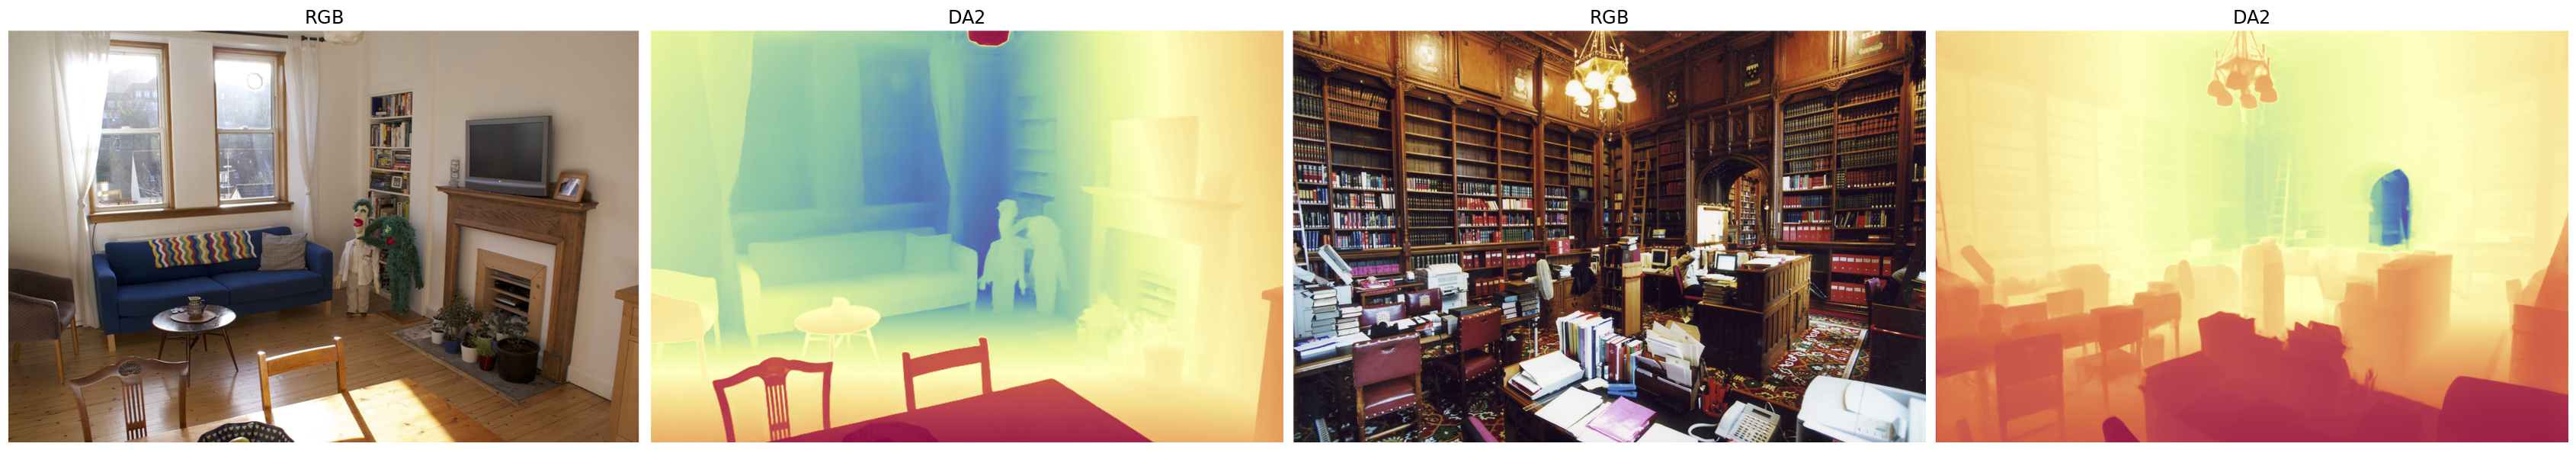
\includegraphics[width=\linewidth]{depth_anything_v2_demo.png}
		\end{column}
	\end{columns}

	\source{Yang et al., arXiv 2024}
\end{frame}


% ==========================================================================
\section{Mathematics}
% ==========================================================================

\sectionslide{QueensGold}{Mathematical Framework}

% --------------------------------------------------------------------------
% SCRIPT: "We formalize the problem as a POMDP. The robot receives partial
% observations --- proprioception and some form of terrain sensing --- and
% outputs 12 joint position offsets. The objective is to maximize expected
% discounted return."
\begin{frame}{Problem Formulation: POMDP}

	\textbf{Partially Observable Markov Decision Process}
	$(\mathcal{S},\, \mathcal{A},\, \mathcal{O},\, T,\, R,\, \gamma)$

	\vspace{10pt}

	\begin{columns}[T]
		\begin{column}{0.48\linewidth}
			\textbf{Observations}
			\begin{itemize}
				\item Proprioception $o_\mathrm{prop} \in \R^{53}$\\
				      {\small angular vel., gravity, joints, contacts}
				\item Exteroception $o_\mathrm{ext}$\\
				      {\small scandots $\R^{132}$ or depth image}
			\end{itemize}
		\end{column}
		\begin{column}{0.48\linewidth}
			\textbf{Actions}
			\begin{itemize}
				\item Joint offsets $a_t \in \R^{12}$
				\item PD controller: $\tau = K_p(a_t - q) - K_d\dot{q}$
			\end{itemize}

			\vspace{8pt}
			\textbf{Objective}
			\[
				J(\pi) = \E_\pi\!\left[\sum_{t=0}^{\infty} \gamma^t R(s_t, a_t)\right]
			\]
		\end{column}
	\end{columns}

\end{frame}

% --------------------------------------------------------------------------
% SCRIPT: "The teacher is trained with PPO. The key idea: instead of
% constraining the KL divergence like TRPO, PPO clips the probability ratio
% to prevent destructive updates. The advantage is estimated with GAE, which
% interpolates between high-bias and high-variance estimates via lambda."
\begin{frame}{PPO: How the Teacher Learns}

	\textbf{Clipped surrogate objective}
	\[
		L^{\mathrm{CLIP}} = \E_t\!\left[\min\!\left(
			r_t\,\hat{A}_t,\;\;
			\clip(r_t,\, 1{-}\epsilon,\, 1{+}\epsilon)\;\hat{A}_t
			\right)\right]
	\]

	\vspace{4pt}
	{\small $r_t = \pi_\theta(a_t|o_t)\,/\,\pi_{\theta_\mathrm{old}}(a_t|o_t)$ \hfill
		Clip prevents large, destructive updates}

	\vspace{14pt}

	\textbf{Generalized Advantage Estimation (GAE)}
	\[
		\hat{A}_t^{\,\mathrm{GAE}(\gamma,\lambda)}
		= \sum_{l=0}^{\infty} (\gamma\lambda)^l\,\delta_{t+l},
		\qquad
		\delta_t = r_t + \gamma V(s_{t+1}) - V(s_t)
	\]

	\vspace{4pt}
	{\small $\lambda$ interpolates: $\lambda{=}0$ (low variance, high bias)
		$\;\leftrightarrow\;$ $\lambda{=}1$ (high variance, low bias)}

	\source{Schulman et al., arXiv 2017; Schulman et al., ICLR 2016}
\end{frame}

% --------------------------------------------------------------------------
% SCRIPT: "The student learns via DAgger. The problem with simple behavioral
% cloning is error compounding --- small mistakes push you off the training
% distribution and errors snowball. DAgger fixes this: the student acts in
% the environment, but the teacher provides the correct labels. The loss has
% two terms: matching the teacher's actions and predicting the correct heading."
\begin{frame}{DAgger: How the Student Learns}

	\textbf{Problem with behavioral cloning:} errors compound under
	distribution shift.

	\vspace{10pt}

	\textbf{DAgger} --- student acts, teacher labels, iterate:
	\[
		\mathcal{L} =
		\underbrace{\|a_\mathrm{teacher} - a_\mathrm{student}\|_2}_{\text{action loss}}
		\;+\;
		\underbrace{\|y_\mathrm{oracle} - \hat{y}\|_2}_{\text{heading loss}}
	\]

	\vspace{10pt}

	{\small The student runs in the environment and collects its own observations,\\
		but the teacher's actions are executed --- eliminating distribution mismatch.}

	\source{Ross et al., AISTATS 2011}
\end{frame}


% ==========================================================================
\section{System}
% ==========================================================================

\sectionslide{QueensRed}{System Architecture}

% --------------------------------------------------------------------------
% SCRIPT: "Here's the full pipeline. Stage 1: the teacher trains with PPO
% using privileged scandot heightmaps. Stage 2: the student replaces scandots
% with depth images and learns via DAgger, with the teacher's actor MLP
% shared between both stages."
\begin{frame}{Two-Stage Pipeline}

	\begin{center}
		\resizebox{0.82\linewidth}{!}{%
			% Pipeline diagram: two-stage teacher-student distillation
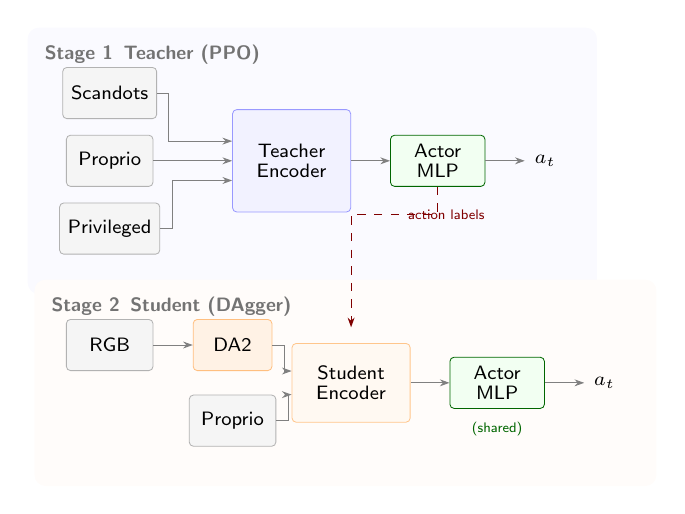
\begin{tikzpicture}[
  >=Stealth,
  % --- shared block base ---
  blkbase/.style={
    rounded corners=1.5pt, minimum height=6.5mm,
    inner xsep=3pt, inner ysep=1.5pt,
    line width=0.3pt, align=center, font=\scriptsize\sffamily
  },
  % --- block types ---
  inp/.style={blkbase, draw=black!30, fill=gray!8, minimum width=11mm},
  da2/.style={blkbase, draw=orange!50, fill=orange!10, minimum width=10mm},
  tenc/.style={blkbase, draw=blue!40, fill=blue!5, minimum width=15mm, minimum height=13mm},
  senc/.style={blkbase, draw=orange!45, fill=orange!5, minimum width=15mm, minimum height=10mm},
  act/.style={blkbase, draw=green!40!black, fill=green!5, minimum width=12mm},
  % --- labels ---
  outlbl/.style={font=\scriptsize\sffamily},
  stglbl/.style={font=\scriptsize\sffamily\bfseries, text=black!55, anchor=north west},
  annot/.style={font=\tiny\sffamily},
  % --- arrows ---
  arr/.style={-{Stealth[length=3.5pt, width=2.5pt]}, line width=0.35pt, draw=black!50},
  darr/.style={-{Stealth[length=3.5pt, width=2.5pt]}, line width=0.4pt, dashed, draw=red!50!black},
]

% ===================== STAGE 1: TEACHER =====================

\node[inp] (scan) at (0, 0) {Scandots};
\node[inp, below=2mm of scan] (prop1) {Proprio};
\node[inp, below=2mm of prop1] (priv) {Privileged};

\node[tenc, right=10mm of prop1] (te) {Teacher\\[-1pt]Encoder};
\node[act] (ta) at ([xshift=11mm]te.east) {Actor\\[-1pt]MLP};
\node[outlbl, right=5mm of ta] (tout) {$a_t$};

\draw[arr] (scan.east) -- ++(1.5mm,0) |- ([yshift=2.5mm]te.west);
\draw[arr] (prop1) -- (te);
\draw[arr] (priv.east) -- ++(1.5mm,0) |- ([yshift=-2.5mm]te.west);
\draw[arr] (te) -- (ta);
\draw[arr] (ta) -- (tout);

% Stage 1 background
\begin{scope}[on background layer]
  \node[draw=none, fill=blue!2, rounded corners=4pt,
    fit=(scan)(priv)(tout), inner xsep=4mm, inner ysep=5mm] (s1) {};
  \node[stglbl] at ([xshift=1mm, yshift=-1mm]s1.north west)
    {Stage 1\enspace Teacher (PPO)};
\end{scope}

% ===================== STAGE 2: STUDENT =====================

\node[inp] (rgb) at (0, -3.2) {RGB};
\node[da2, right=5mm of rgb] (d2) {DA2};
\node[inp, below=3mm of d2] (prop2) {Proprio};

\node[senc] (se) at ([xshift=10mm]d2.east |- {$(d2)!0.5!(prop2)$}) {Student\\[-1pt]Encoder};
\node[act] (sa) at ([xshift=11mm]se.east) {Actor\\[-1pt]MLP};
\node[outlbl, right=5mm of sa] (sout) {$a_t$};

\draw[arr] (rgb) -- (d2);
\draw[arr] (d2.east) -- ++(1.5mm,0) |- ([yshift=1.5mm]se.west);
\draw[arr] (prop2.east) -- ++(1.5mm,0) |- ([yshift=-1.5mm]se.west);
\draw[arr] (se) -- (sa);
\draw[arr] (sa) -- (sout);

% Stage 2 background
\begin{scope}[on background layer]
  \node[draw=none, fill=orange!2, rounded corners=4pt,
    fit=(rgb)(prop2)(sout), inner xsep=4mm, inner ysep=5mm] (s2) {};
  \node[stglbl] at ([xshift=1mm, yshift=-1mm]s2.north west)
    {Stage 2\enspace Student (DAgger)};
\end{scope}

% ===================== CONNECTIONS =====================

% DAgger supervision arrow
\draw[darr]
  (ta.south) -- ++(0,-3.5mm)
  -| node[pos=0.25, right=0.5mm, annot, text=red!50!black] {action labels}
  ([yshift=2mm]se.north);

% Shared actor annotation
\node[annot, text=green!40!black, below=0.5mm of sa] {(shared)};

\end{tikzpicture}
%
		}
	\end{center}

	\vspace{4pt}
	{\small Stage 1: Teacher trains with privileged scandots (PPO)\\
		Stage 2: Student imitates from depth images (DAgger), shared actor MLP}

\end{frame}

% --------------------------------------------------------------------------
% SCRIPT: "The student's visual encoder: a CNN maps the depth image to a
% 32-dimensional feature, fused with proprioception, then processed by a GRU
% that integrates over time to produce the terrain latent and heading estimate."
\begin{frame}{Student Visual Encoder}

	\begin{center}
		\resizebox{0.85\linewidth}{!}{%
			% Student visual encoder architecture
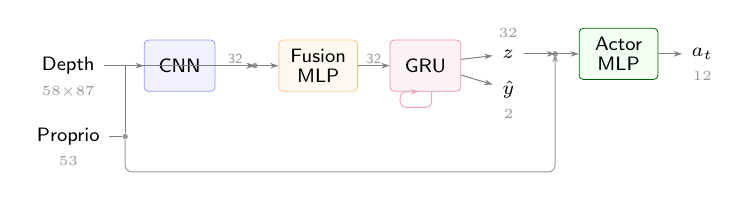
\begin{tikzpicture}[
  >=Stealth,
  % --- shared block base ---
  blkbase/.style={
    rounded corners=1.5pt, minimum height=6.5mm,
    inner xsep=2.5pt, inner ysep=1.5pt,
    line width=0.3pt, align=center, font=\scriptsize\sffamily
  },
  % --- block types ---
  cnn/.style={blkbase, draw=blue!40, fill=blue!5, minimum width=9mm},
  fuse/.style={blkbase, draw=orange!45, fill=orange!5, minimum width=10mm},
  gru/.style={blkbase, draw=purple!40, fill=purple!5, minimum width=9mm},
  act/.style={blkbase, draw=green!40!black, fill=green!5, minimum width=10mm},
  % --- labels ---
  io/.style={font=\scriptsize\sffamily},
  dim/.style={font=\tiny\sffamily, text=black!40, inner sep=0.5pt},
  % --- arrows ---
  arr/.style={-{Stealth[length=3pt, width=2pt]}, line width=0.35pt, draw=black!50},
]

% ===================== INPUTS =====================

\node[io] (depth) at (0, 0.4) {Depth};
\node[dim, below=0mm of depth] {$58{\times}87$};

\node[io] (prop) at (0, -0.5) {Proprio};
\node[dim, below=0mm of prop] {$53$};

% ===================== PROCESSING =====================

\node[cnn, right=5mm of depth] (cnn) {CNN};

% Concat point 1
\coordinate (cat1) at ([xshift=5mm]cnn.east);
\node[circle, fill=black!40, inner sep=0.7pt] at (cat1) {};

\node[fuse, right=3mm of cat1] (fmlp) {Fusion\\[-1pt]MLP};

\node[gru, right=4mm of fmlp] (gru) {GRU};

% GRU recurrence
\draw[arr, rounded corners=2pt, draw=purple!35]
  ([xshift=0.8mm]gru.south) -- ++(0,-2mm) -- ++(-4mm,0) -- ++(0,2mm)
  -- ([xshift=-0.8mm]gru.south);

% ===================== GRU OUTPUTS =====================

\node[io, right=4mm of gru, yshift=1.5mm] (z) {$z$};
\node[dim, above=0mm of z] {$32$};
\node[io, right=4mm of gru, yshift=-3mm] (yhat) {$\hat{y}$};
\node[dim, below=0mm of yhat] {$2$};

% Concat point 2
\coordinate (cat2) at ([xshift=4mm]z.east);
\node[circle, fill=black!40, inner sep=0.7pt] at (cat2) {};

\node[act, right=3mm of cat2] (actor) {Actor\\[-1pt]MLP};

\node[io, right=3mm of actor] (out) {$a_t$};
\node[dim, below=0mm of out] {$12$};

% ===================== ARROWS =====================

\draw[arr] (depth) -- (cnn);
\draw[arr] (cnn) -- node[dim, above] {32} (cat1);
\draw[arr] (cat1) -- (fmlp);
\draw[arr] (fmlp) -- node[dim, above] {32} (gru);
\draw[arr] ([yshift=0.8mm]gru.east) -- (z);
\draw[arr] ([yshift=-1.2mm]gru.east) -- (yhat);
\draw[arr] (z) -- (cat2);
\draw[arr] (cat2) -- (actor);
\draw[arr] (actor) -- (out);

% Proprio branch point
\node[circle, fill=black!40, inner sep=0.7pt] (pbr) at ([xshift=2mm]prop.east) {};

% Branch 1: to fusion
\draw[arr] (prop.east) -- (pbr) |- (cat1);

% Branch 2: to actor (route below)
\draw[arr, rounded corners=2.5pt, draw=black!40]
  (pbr) -- ++(0,-4.5mm) -| (cat2);

\end{tikzpicture}
%
		}
	\end{center}

	\vspace{6pt}
	{\small Depth CNN $\to$ Fusion MLP $\to$ GRU $\to$ terrain latent $z \in \R^{32}$
		+ heading $\hat{y} \in \R^{2}$}

\end{frame}

% --------------------------------------------------------------------------
% SCRIPT: "We test on three obstacle families --- stairs, hurdles, and gaps ---
% at four difficulty levels each. These are simpler than prior work; our goal
% is to isolate the vision question, not push agility."
\begin{frame}{Terrain and Curriculum}

	\begin{center}
		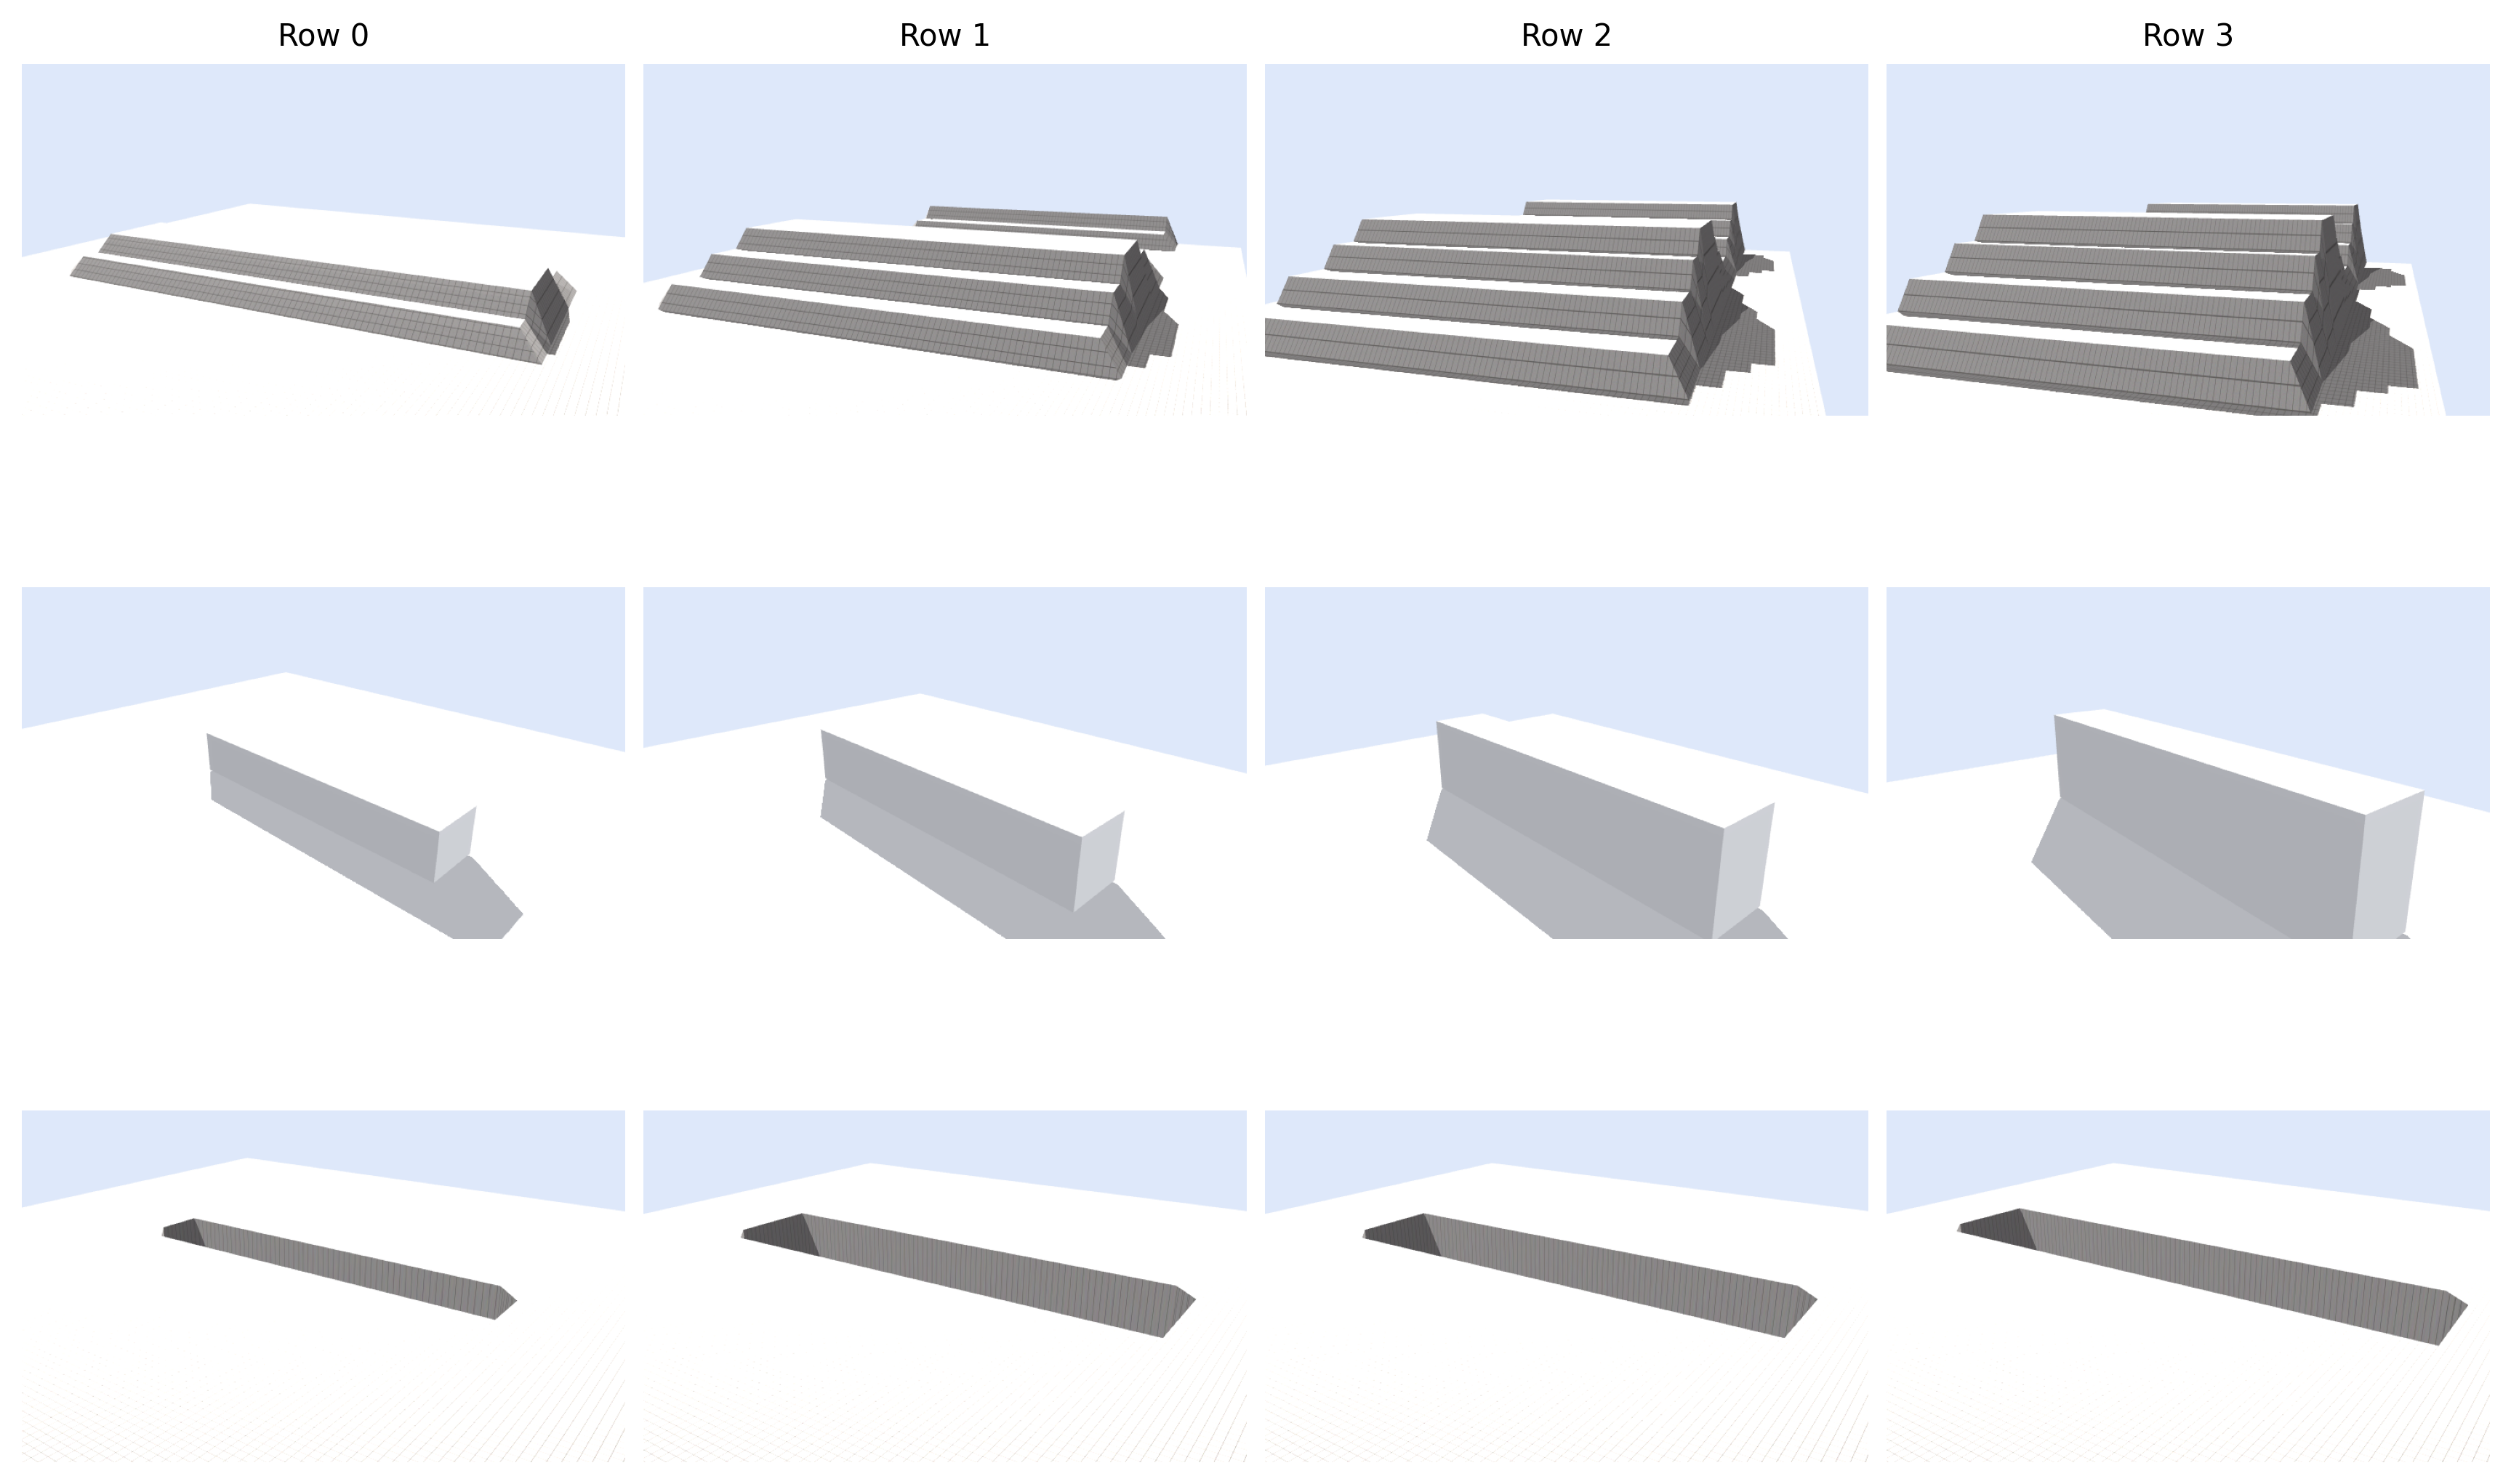
\includegraphics[width=0.85\linewidth]{terrain_curriculum.png}
	\end{center}

	\vspace{2pt}
	{\small Three obstacle families $\times$ four difficulty levels.
		Deliberately simpler than prior work --- isolating the depth estimation question.}

\end{frame}

% --------------------------------------------------------------------------
% SCRIPT: "Let me show you what this looks like in practice."
\begin{frame}[plain,c]

	\begin{center}
		{\Large\bfseries Simulation Demo}

		\vspace{16pt}

		% [PLACEHOLDER] Embed video or animated GIF here
		\placeholder[0.2\textheight]{Video demo --- show simulation runs here}
	\end{center}

\end{frame}


% ==========================================================================
\section{Results}
% ==========================================================================

\sectionslide{QueensBlue}{Experiments \& Results}

% --------------------------------------------------------------------------
% SCRIPT: "First, we establish upper bounds. The teacher with privileged
% scandots hits 99 percent. The GT-depth student --- trained on perfect
% simulator depth --- reaches about 90 percent. A zero-depth ablation drops
% to 8 percent, confirming the policy actually relies on depth, not
% proprioceptive heuristics. The architecture works. Depth quality is the
% bottleneck."
\begin{frame}{Baselines: Upper Bounds}

	\begin{center}
		\begin{tabular}{@{}lcccc@{}}
			\toprule
			                    & Row~0 & Row~1 & Row~2 & Row~3 \\
			\midrule
			Scandots teacher    & 98.5  & 100.0 & 99.0  & 98.5  \\
			GT-depth student    & 94.5  & 94.5  & 89.1  & 87.5  \\
			Zero-depth ablation & 8.0   & 2.0   & 0.0   & 0.0   \\
			\bottomrule
		\end{tabular}
	\end{center}

	\vspace{12pt}

	\begin{center}
		The student architecture works.\\
		\textbf{Depth quality} is the bottleneck, not the network.
	\end{center}

\end{frame}

% --------------------------------------------------------------------------
% SCRIPT: "Now we replace simulator depth with DA2 estimates. DA2-small fails
% on hard gaps. DA2-base gets further but drops off sharply on rows 2 and 3.
% The key finding: adding checkerboard texture to the terrain closes most of
% the remaining gap. The depth estimator needs visual features to find obstacle
% boundaries."
\begin{frame}{Estimated Depth: Model Scale and Texture}

	\begin{columns}[T]
		\begin{column}{0.48\linewidth}
			\small
			\begin{tabular}{@{}lcccc@{}}
				\toprule
				             & R0 & R1 & R2  & R3  \\
				\midrule
				DA2-small    & 56 & 34 & --- & --- \\
				DA2-base     & 68 & 83 & 27  & 1   \\
				DA2-base+tex & 65 & 64 & 68  & 45  \\
				\midrule
				GT-depth     & 95 & 95 & 89  & 88  \\
				\bottomrule
			\end{tabular}

			\vspace{8pt}
			Larger model + texture\\$\to$ closes gap to GT-depth
		\end{column}
		\begin{column}{0.5\linewidth}
			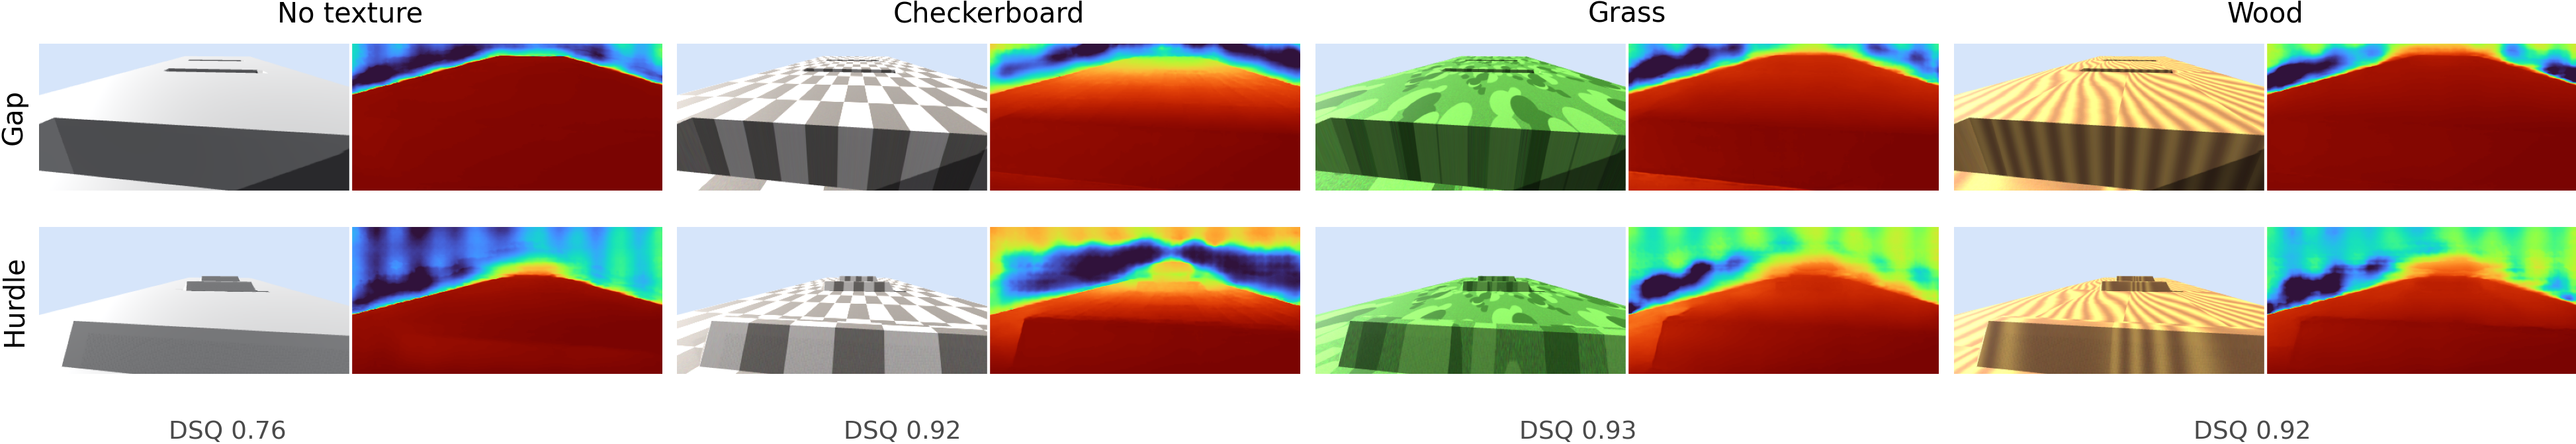
\includegraphics[width=\linewidth]{da2_texture_comparison.png}
		\end{column}
	\end{columns}

\end{frame}

% --------------------------------------------------------------------------
% SCRIPT: "We introduced DSQ --- Depth Signal Quality --- as a diagnostic.
% It's the Pearson correlation between ground-truth and estimated depth,
% averaged over frames. Because Pearson correlation is affine invariant,
% it naturally handles the scale ambiguity in monocular depth."
\begin{frame}{Depth Signal Quality (DSQ)}

	A diagnostic metric: how well does estimated depth preserve terrain geometry?

	\vspace{10pt}

	\[
		\mathrm{DSQ} = \frac{1}{T}\sum_{t=1}^{T}
		\frac{1}{N}\sum_{i=1}^{N}
		\rho\!\left(d_i^{\,\mathrm{GT}},\; d_i^{\,\mathrm{DA2}}\right)
	\]

	\vspace{10pt}

	{\small Pearson correlation is \textbf{affine invariant}:
		$\rho(\alpha x + \beta,\, y) = \rho(x,y)$\\[2pt]
		$\to$ naturally handles monocular scale--shift ambiguity}

\end{frame}

% --------------------------------------------------------------------------
% SCRIPT: "Finally, we perturbed visual appearance at test time: texture
% swaps, lighting changes, color shifts, and combined perturbations. The DSQ
% scatter plot tells the story. Low DSQ means failure. But high DSQ alone
% doesn't guarantee success --- some unseen textures still fool the policy.
% Stairs and hurdles are robust because they have strong edges. Gaps are the
% most fragile because their boundaries depend on surface texture."
\begin{frame}{Visual Sensitivity}

	\begin{columns}[T]
		\begin{column}{0.52\linewidth}
			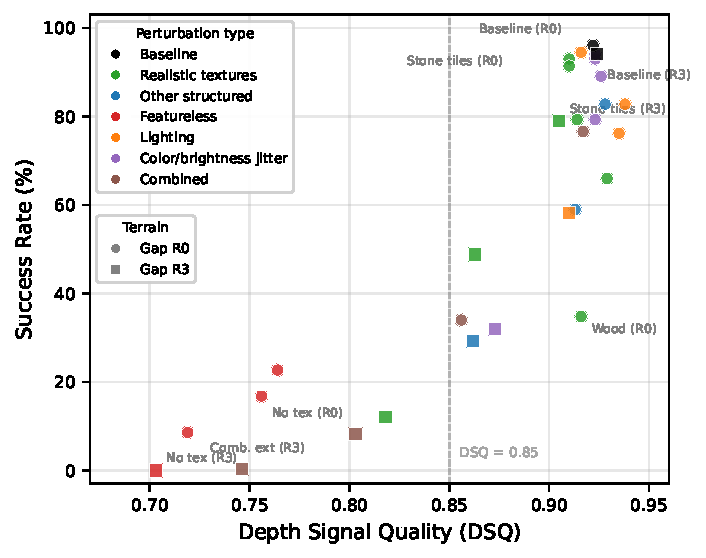
\includegraphics[width=\linewidth]{dsq_scatter.pdf}
		\end{column}
		\begin{column}{0.44\linewidth}
			\vspace{8pt}
			\begin{itemize}
				\item Stairs/hurdles: robust\\
				      {\small (strong geometric edges)}
				\item Gaps: fragile\\
				      {\small (boundary depends on texture)}
				\item Featureless $\to$ catastrophic
				\item Lighting/color $\to$ moderate
			\end{itemize}

			\vspace{8pt}
			{\small DSQ predicts failure well,\\
				but high DSQ $\neq$ guaranteed success}
		\end{column}
	\end{columns}

\end{frame}


% ==========================================================================
\section{Conclusion}
% ==========================================================================

\sectionslide{QueensGold}{Takeaways}

% --------------------------------------------------------------------------
% SCRIPT: "So what did we learn? Monocular depth estimation is a plausible
% bridge from RGB to locomotion. The bottleneck is depth quality, not the
% student architecture. DA2 is robust to photometric variation --- lighting,
% color --- but fragile on featureless or weak-texture surfaces. The next
% step is real-world transfer on the Go2, along with temporal depth models
% that might stabilize frame-to-frame predictions."
\begin{frame}{What We Learned}

	\begin{enumerate}
		\item Monocular depth is a \textbf{plausible bridge} from RGB to locomotion
		\item Bottleneck = \textbf{depth quality}, not student architecture
		\item Robust to photometric variation; \textbf{fragile on featureless surfaces}
	\end{enumerate}

	\vspace{14pt}

	\textbf{Future work}
	\begin{itemize}
		\item Real-world transfer on Unitree Go2
		\item Temporally consistent depth models
		\item Joint adaptation of depth estimator + student policy
	\end{itemize}

\end{frame}


% ==========================================================================
% CLOSING
% ==========================================================================

\sectionslide{QueensBlue}{Thank you! \\[1em]Questions?}

\end{document}
